\section{Introduction}

\subsection{Definition}

\begin{definition}[Negotiation]
    \begin{itemize}
        \item "By negotiation we mean exchange between parties designed to reconcile
            their differences and produce a settlement" (Brams 2003)
        \item "Negotiation - a process involving multiple individuals cooperating to
            arrive at a joint decision. The joint decision entails joint consequences,
            or payoffs, for each individual." (Raiffa 2003)
        \item "Like it or not, but you are a negotiatior. Negotiation is a fact
            of life. Everyone negotiates something every day" (Fisher and Ury 2012)
    \end{itemize}
\end{definition}

\paragraph{Common things in Negotiations}
\begin{itemize}
    \item There are 2 or more parties (special case: 1 person against "nature")
    \item Conflict of needs
    \item Choice
    \item Give-and-take process
    \item Prefer to negotiate rather than to "fight openly"
    \item "Tangibles" and "Intangibles" ("Materialles" und "Immaterielles")
\end{itemize}

\paragraph{When should people, in normal cases, \underline{not} participate in negotiation?}
\begin{itemize}
    \item No willingness to make concession
    \item Demands are unethical*
    \item The other side acts in bad faith*
    \item You are not prepared*
\end{itemize}
\hspace{15pt} * = exeptions possible

\begin{definition}[Mediation]
    "Any action taken by an actor tat is not a direct party to the crisis, that is
    designed to reduce or remove one or more of the problems of the bargaining
    relationship, and therefore to facilitate the termination of the crisis itself."
    (Oran Young)
\end{definition}

\subsection{Taxonomy (Negotiation)}

\begin{figure}[h]
    \centering
    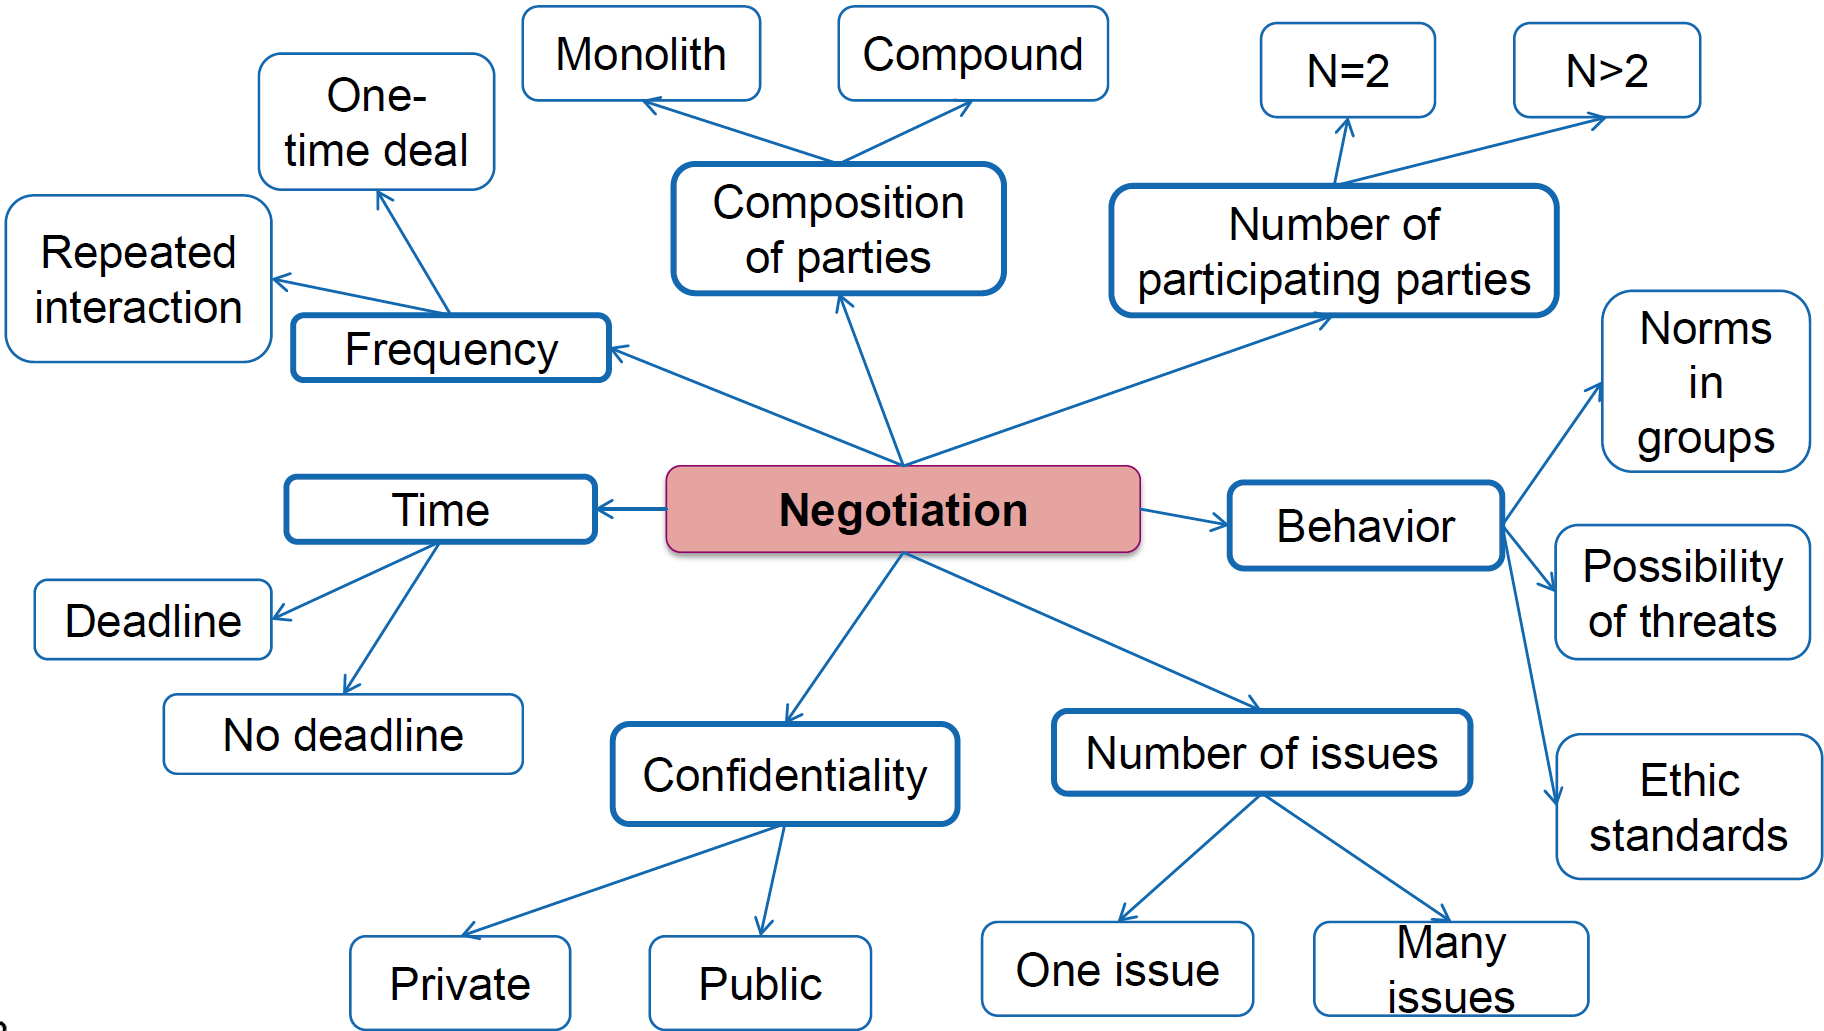
\includegraphics[width=0.5\textwidth]{Pictures/Taxonomy_General.png}
    \label{fig:Taxonomy_General}
\end{figure}

\begin{definition}[Distributive Negotiation]
    Distributive negotiation is a competitive negotiation over one issue, a win-lose
    situation, such as haggling over a price in a bazar. It is adversarial.
    Revealing information can be a handicap for a party.
\end{definition}

\begin{definition}[Integrative Negotiation]
    Integrative negotiation is a negotiation that can look for win-win solutions
    or problem solving in order to have mutual gain. It is cooperative. Sharing
    information is helpful/necessary for both parties.
\end{definition}

\begin{figure}[H]
    \centering
    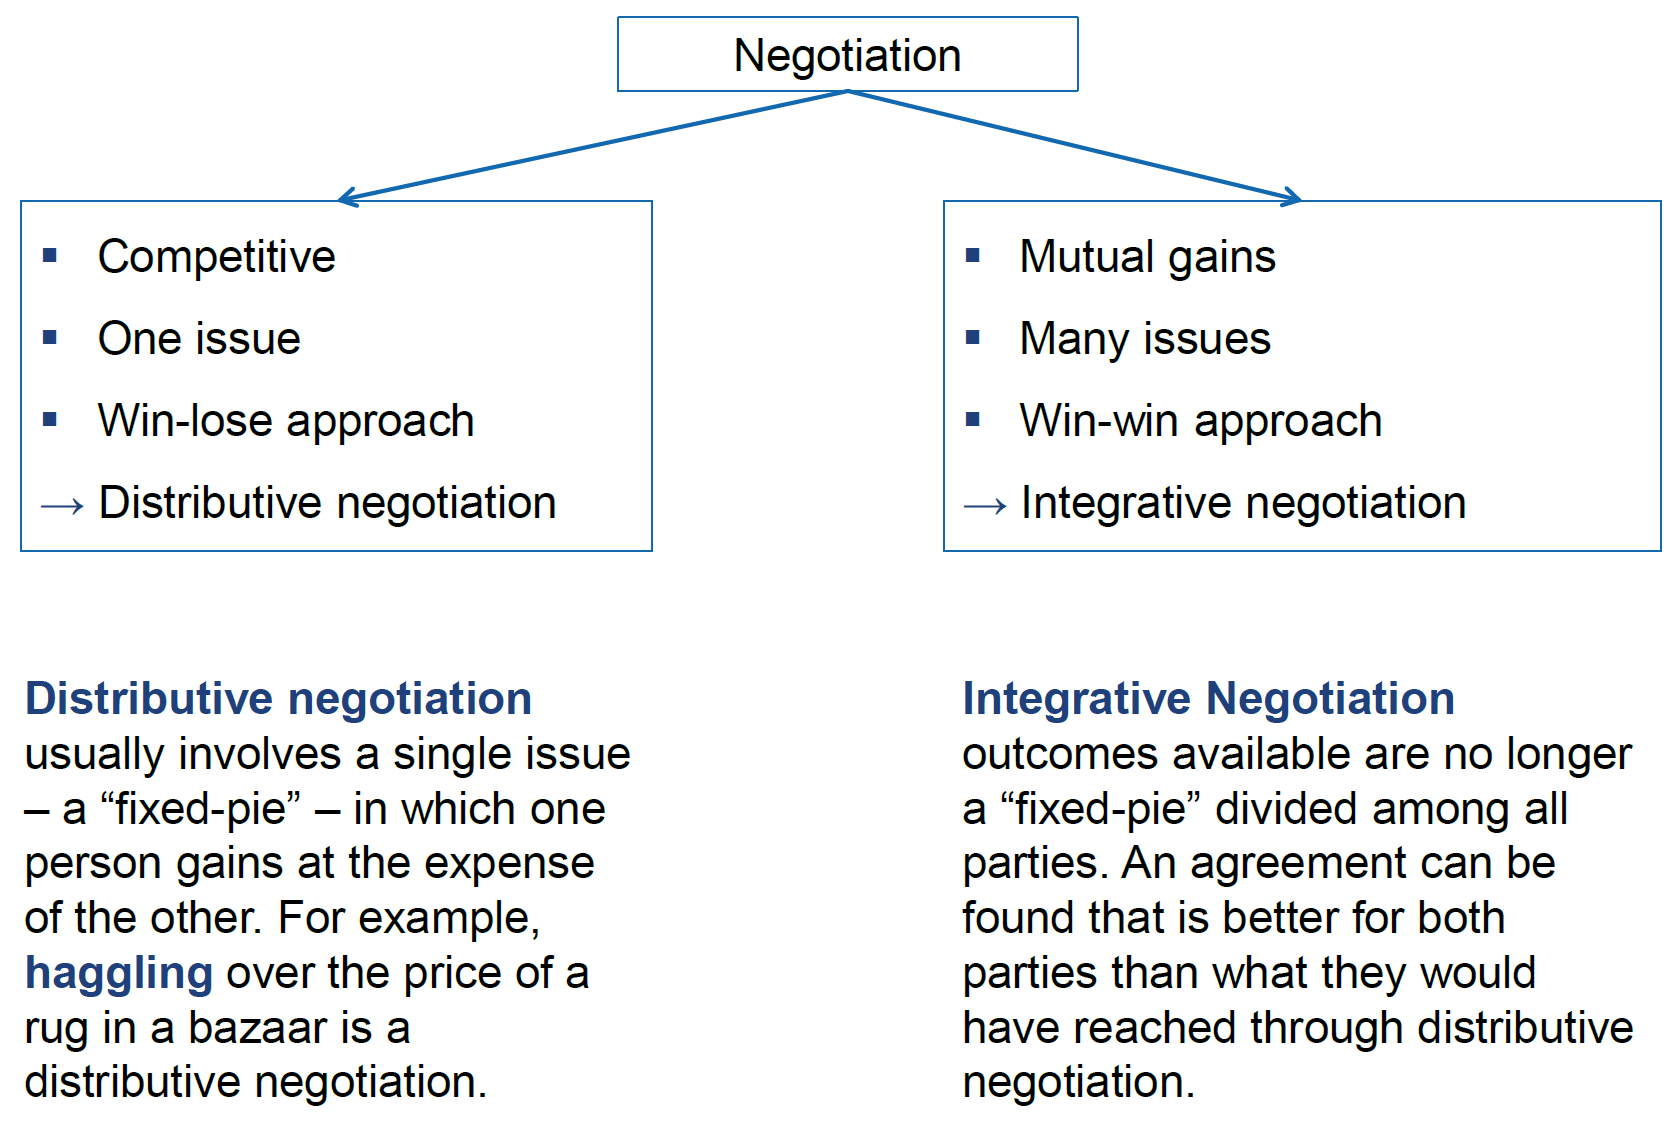
\includegraphics[width=0.5\textwidth]{Pictures/Distributive_vs_Integrative_Negotiation.png}
    \caption{Distributive vs. Integrative Negotiation}
    \label{Distributive_vs_Integrative_Negotiation}
\end{figure}

\subsubsection{Negotiation and decision Theory}

\begin{figure}[H]
    \centering
    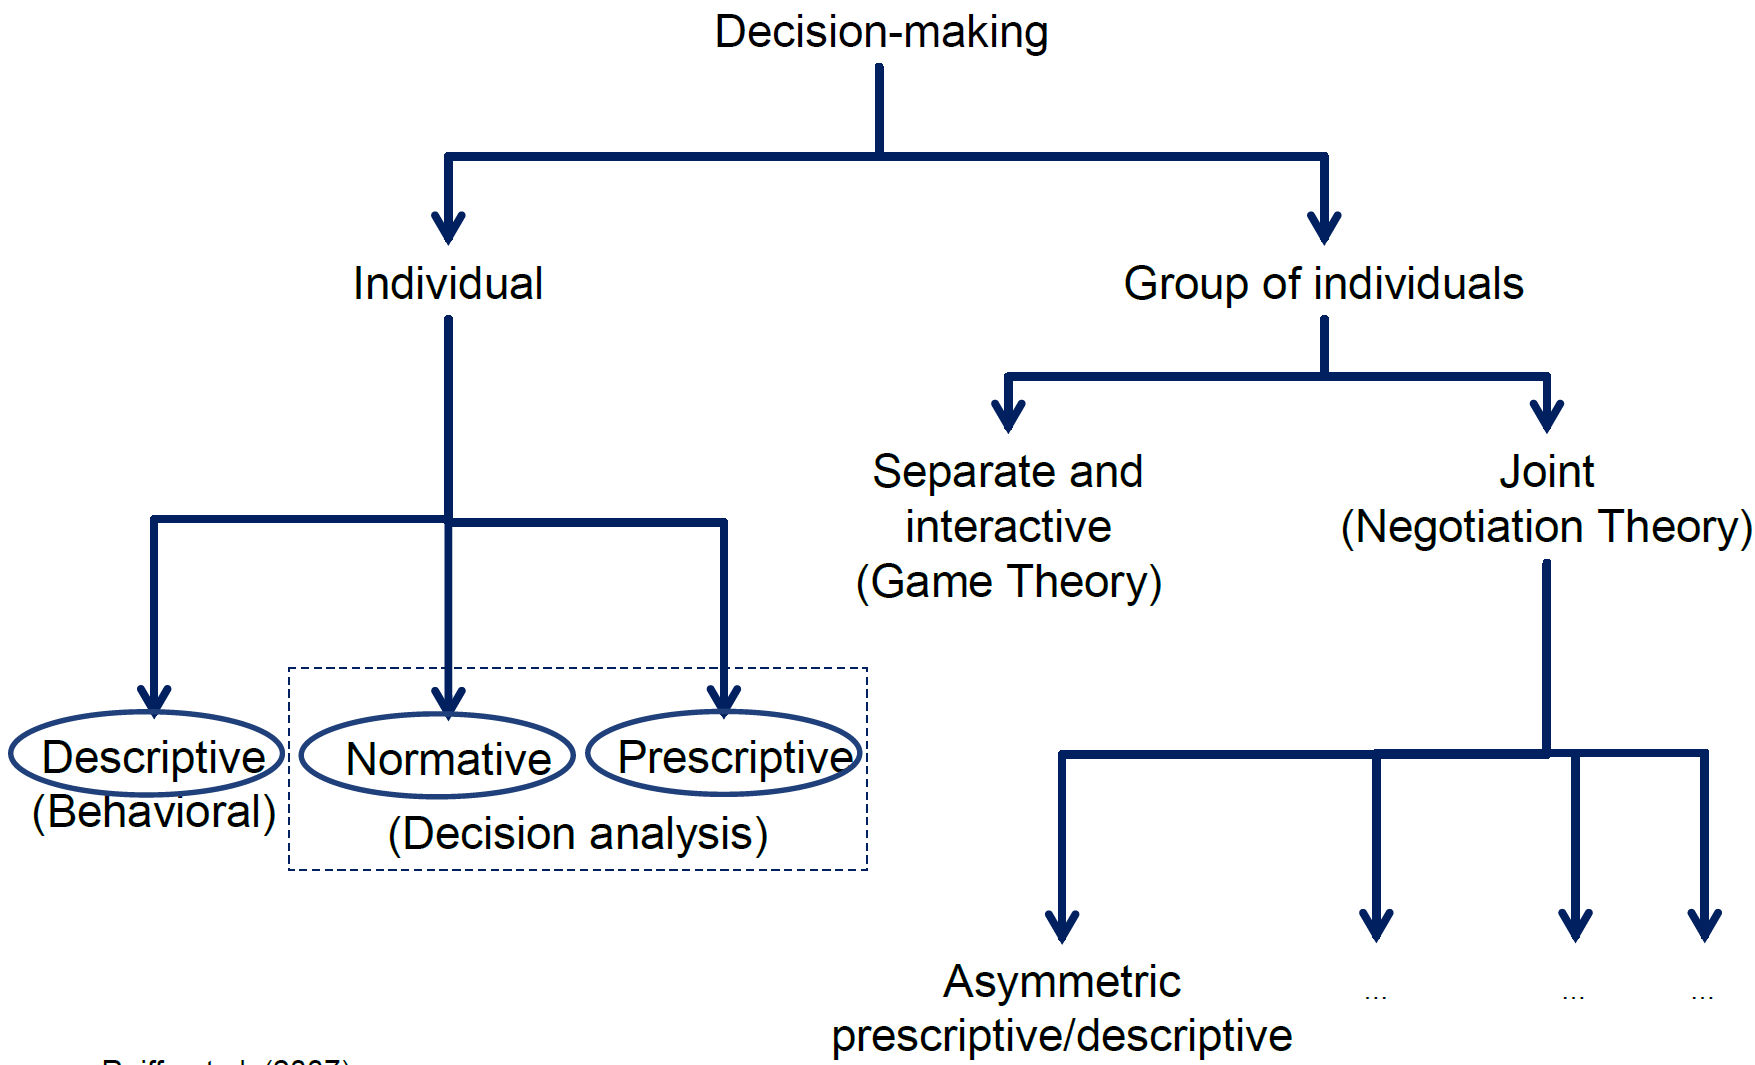
\includegraphics[width=0.5\textwidth]{Pictures/Negotiation_and_decision_theory.png}
    \label{Negotiation_and_decision_theory}
\end{figure}

\paragraph{Descriptive, normative, and prescriptive orientations}
\begin{itemize}
    \item \underline{Descriptive}: How decisions are made. How and why individuals
        think and act the way they do.
    \item \underline{Normative}: How decisions should be made. How idealized, rational,
        super-intelligent people should act. Often used in applied mathematics
        because concept is clear. However, normative theories $\rightarrow$ often
        only first-order approximations of real-world behaviour.
    \item \underline{Prescriptive}: How decisions could be made better. What can a
        real person actually do to make better decisions? What is practically useful?
\end{itemize}

\subsection{Rationality}

\subsubsection{Definition}

\begin{definition}[Rationality]
    Let $a$ be an action and $a \in A$ (set of alternative actions), $\omega$
    the outcome and $u$ the utility. A utility function is a function
    $u: \Omega \rightarrow \R$ such that $u(\omega_1) > u(\omega_2) \Leftrightarrow
    \omega_1 \succ \omega_2$. A payoff function $\pi: A \rightarrow \R$. $\lambda$
    is a lottery, a set of probablities for the occurence of every $\omega \in \Omega$.
    For the probability that outcome $\omega$ occurs in lottery $\lambda$ we denote
    $p(\omega | \lambda)$. The expected utility (expected payoff) is
    $\pi(a) = \sum_{\omega \in \Omega} p(\omega | \lambda(a)) \cdot u(\omega)$
\end{definition}

\vspace{1\baselineskip}

An individual is rational under certainty if his preferences for outcomes
$\omega \in \Omega$ satisfy the following conditions:
\begin{enumerate}[1)]
    \item Completeness: Either $\omega_1 \succcurlyeq \omega_2$ or $\omega_2 \succcurlyeq \omega_1$
    \item Transitivity: If $\omega_1 \succcurlyeq \omega_2$ and $\omega_2 \succcurlyeq \omega_3$,
        then $\omega_1 \succcurlyeq \omega_3$.
\end{enumerate}
An individual is rational under uncertainty if his preferences for lotteries satisfy
the following conditions:
\begin{enumerate}[1)]
    \item Completeness: Either $\lambda_1 \succcurlyeq \lambda_2$ or $\lambda_2 \succcurlyeq \lambda_1$
    \item Transitivity: If $\lambda_1 \succcurlyeq \lambda_2$ and $\lambda_2 \succcurlyeq \lambda_3$,
        then $\lambda_1 \succcurlyeq \lambda_3$
    \item Monotonitity: If $\lambda_1 \succ \lambda_2$ and $q_1 > q_2$, then
        $q_1 \lambda_1 + (1-q_1) \lambda_2 \succ q_2 \lambda_1 + (1-q_2) \lambda_2$
    \item Continuity: If $\lambda_1 \succcurlyeq \lambda_2$ and $\lambda_2 \succcurlyeq \lambda_3$,
        then there exists a probability $q$ such that $\lambda_2 \sim q \lambda_1 + (1-q) \lambda_3$
    \item Independence: If $\lambda_1 \succ \lambda_2$, then $q \lambda_1 + (1-q) \lambda_2
        \succ q \lambda_2 + (1-q) \lambda_3$
\end{enumerate}

\vspace{1\baselineskip}

\begin{definition}[Transitivity]
    A relation $R$ is transitive, if $\forall a,b,c \in A: (a,b) \in R \wedge
    (b,c) \in R \Rightarrow (a,c) \in R$
\end{definition}

\vspace{1\baselineskip}

Non-Transitivity creates a perpetuum mobile. Transitivity is an important
condition for rational behaviour. It is a concept in the normative orientation.
However, in exeptional cases it can also lead to problems/paradoxes.

\vspace{1\baselineskip}

\begin{definition}[Behaving rationally]
    The negotiation objecitves are based on comprehensible motivations and
    the measures to achieve these objecitves are consistent and do not violate
    generally acceptable conventions/customs.
\end{definition}

\vspace{1\baselineskip}

Negotiation parties representing a big group, will be considered as behaving
rationally if the negotiation is conducted/monitored
\begin{itemize}
    \item by professional people of the negotiation party
    \item of which a couple of people (i.e. more than 5) are not directly
        participating in the negotiation but work in a sort of "back-office" function.
    \item where the work culture permits an internal objective/critical discussion.
\end{itemize}

\subsection{Brief excursion to philosophical concepts}

A big question of moral and political philosophy: Is morality a matter of
counting lives and weighing costs and benefits, depending solely on the consequences
it brings about or are certain moral duties and human rights so fundamental that they
rise above such calculations, for reasons independent of the social consequences?

\paragraph{Utilitarianism}

"The highest principle of morality is to maximize happiness, the overlal balance
of pleasure over pain."
"The greatest good for the greatest number" was the ethic system.

Objections: Utilitarianism fails to respect individual rights. Difficult to
translate all moral goods into a single currency of value (utility function).

Criticism: Only actions done due to a motive of duty (doing something because
it is right) have moral worth. The moral worth of an action is dependent on the
motive from which it is done, not the results it produces.

Kant developed the Categorical Imperative (universal law): "Act only according
to the maxim whereby you can, at the same time, will that it should become a
universal law"
